\documentclass[11pt, english, a4paper]{report-rd-info}
   % - 12pt:  can be preferable to read the report on small screens, ask your supervisors
   % - screen:  to be removed in order to obtain a classical report
\usepackage[latin1]{inputenc}
   % - latin9, utf8, etc.
\usepackage[T1]{fontenc}

% some definitions for the actual contents
\usepackage{enumerate}
\usepackage{amsmath, amssymb}
\usepackage{algorithm,algpseudocode}
%\usepackage{algorithmic}
\usepackage{color}
\usepackage{graphicx}

\begin{document}

\title{Massive Broadcasting with WebRTC}
\subtitle{An evaluation of peer-to-peer networks with handshakes}

\authorA{Julian}{Tanke}
\authorB{}{}
\supervisor{Pascal}{Molli}
\cosupervisor{Brice}{Nedelec}
   % In case, there are more than two supervisors, use the following trick:
   %    \cosupervisor{Jean}{Cadre \& {\normalfont Still} Another}
\coordinator{Jos�}{Martinez}
\institution{LINA}
   % - LINA when you're supervised by members of the research teams GRIM or COD (may be some others);
   % - IRCCyN when youre supervised by members of the research team IVC;
   % - XXX when supervised by another organism
   %   (In that case, you have to provide, in the "logos" directories, the files named: XXX.pdf -- if not XXX.jpeg or XXX.png -- for pdflatex *and* XXX.eps for latex);
   % - otherwise comment it
\theme{\'Equipe GRIM}
   % - optionally provide it when an institution has been declared (GRIM, COD or IVC for the local research teams)
   % - otherwise comment it
%\coinstitution{Centre national de la recherche scientifique}{CNRS}{1.7cm}
   % - if you need to add a partner
   % - the logo must be provided, e.g., CNRS.pdf here
   % - the third parameter allows one to control the width of the logo in order to make
   %   it look of the same size of the one from the university of nantes and possibly the laboratory
\date{November 15, 2014}
   % - do not had un 0 in front of the first to ninth day of a mont!
   % - you can altogether ignore the day.

%-------------------------------------------------------------------------------------------------------------

\begin{abstract}
%\small % Comment it out should the abstract by slightly too long to fit in the page.
   As the name suggests, the abstract is a very short but informative piece of information about everything you did in this work, i.e., successively the description of the problem at hand, the objectives, the main point of the state-of-the-art, the choices made, the conceptual developments, the conducted experiments, results and interpretations, the new issues.

   It is the last thing to write!
\end{abstract}

\begin{classification}
%\small % Idem
   Bibliographic indexing is required. Use the ACM thesaurus:  See \url{http://www.acm.org/about/class/}. (The following example is based on the 1998 version, where general terms and additional key words are optional.)

   \category{H.2.8}{Database Applications}{Image databases}
   \category{H.3.3}{Information Search and Retrieval}{Clustering, Information filtering, Relevance feedback}
   \category{H.3.7}{Digital Libraries}{User issues}
   \category{I.5.3}{Clustering}{Algorithms, Similarity measures}
   \category{I.4.10}{Image Representation}{Statistical, Multidimensional}
   \terms{Algorithms, Performances, Experiments, Human factors, Verification.}
   \keywords{Content-based image retrieval system, Classification, Feedback loop, Supervised learning.}
\end{classification}

\maketitle

%--------------------------------------------------------------------------------

\begin{acknowledgements}
LSEQ and A Scalable Encoding for Massive Collaborative Editing 
\end{acknowledgements}

%--------------------------------------------------------------------------------

\newpage

\tableofcontents

%--------------------------------------------------------------------------------

\chapter{Introduction}

% 1:Motivation - why interesting and important for larger community?

Many efforts have been devoted to establish data connections between browsers using the WebRTC API\cite{webrtc}.
Services like PeerCDN\cite{peercdn}, webtorrent\cite{webtorrent} or Sharefest\cite{sharefest} demonstrate how decentralized services now can be deployed easily in web browsers.
This improves the user experience drastically as users can download a torrent as easy as watching a youtube video.
However, current solutions do not provide a scalable broadcast.
This, however, is essential for other applications such as distributed collaborative editors or distributed social networks.
Traditionally, gossip protocols are used to implement broadcast in decentralized infrastructure.
This protocols have been used in a various number of large scale systems serving an array of problem settings including information dissemination \cite{Demers:1987:EAR:41840.41841}, information aggregation \cite{Jelasity:2005:GAL:1082469.1082470} and network management \cite{conf/dsom/VoulgarisS03}.
Peers are highly autonomous and independent, which allows the algorithms to be simple when compared to hierarchical approaches.
This protocols can easily scale to millions of peers which can join and leave without significantly disrupting the service.

% 2:What is the specific problem? and background
This raises the problem of deploying gossip algorithms on WebRTC.
Many gossip protocols build up upon the premise that the peers can interconnect easily with each other and, as such, constantly connect to new sets of peers\cite{Voulgaris05cyclon:inexpensive}\cite{Jelasity:2004:PSS:1045658.1045666}.
Unfortunatly, certain efforts must be taken to establish a peer-to-peer connection with WebRTC:
a handshake, consisting of an offer by one client and a responding answer by the other, must be performed.
This process must be hoist by a well-known service in between, which we will call the \emph{signaling service}.
Furthermore, the handshake radically changes the communication complexity as connecting to new peers becomes more expansive and error-prone.

% 3:summarize main contributions. What is the general approach taken? Why significant? MUST BE GOOD!

In this report we evaluate the cost of current gossip algorithms in a WebRTC infrastructure.
We propose a new algorithm that minimizes the number of connections to the well-known signaling service and instead hosts the handshaking inside the protocol.

% 4:High level: what are the differences to what others have done. Reader must know whats new about this work
% to compare to other work in the area

Gossip protocols that are designed for the internet have already been introduced by \cite{Ganesh:2003:PMM:642778.642782} and\cite{Voulgaris03arobust}.
However, this protocols assume that a connection can be established with direct addressing, ignoring the limitations mentioned above.

% 5:structure

The remainder of this paper is structured as follows: 
Chapter~\ref{chap:Motiv} explains the technology in more depth and provides an example application. 
Chapter~\ref{chap:StateOfTheArt} studies a number of gossip protocols. 
In Chapter~\ref{chap:Proposals} we will introduce an example application. 
Furthermore we will outline the requirements for a handshaking gossip protocol.
Chapter~\ref{chap:Experiments} follows a development, experiment, and analysis path in order to quantify the theoretical results.
Finally, the conclusion summarises the work and introduce new research issues that are worth pursuing.

%-------------------------------------------------------------------------------------------------------------

\chapter{Background and Motivation}
\label{chap:Motiv}

\section{WebRTC}

Web Real-Time Communications (WebRTC) is a client-side API to enable Real-Time Communications in web browsers \cite{webrtc}.
It is an implementation of SRTP\footnote{Secure Real-time Transport Protocol} with an SDP\footnote{Sockets Direct Protocol} control mechanism on top that can use STUN, TURN and ICE for NAT traversal.

\textit{These APIs should enable building applications that can be run inside a browser, requiring no extra downloads or plugins, that allow communication between parties using audio, video and supplementary real-time communication, without having to use intervening servers (unless needed for firewall traversal, or for providing intermediary services).}

As we are interested in sending arbitrary data beween peers we will focus on the DataChannel API.
Unfortunately WebRTC cannot create a connection between peers without a signaling service. 
That means that we need some sort of communication exchange (Handshake) prior to the direct peer-to-peer connection.
Figure~\ref{fig:webrtc} demonstrates how a connection is established in WebRTC:

\begin{enumerate}
    \item{Alice needs to find out her public internet address and her network setup (Routers, Firewall).
To obtain this information, she queries a well-known STUN-Server.}
    \item{To establish a connection with Bob, she now needs to create an offer and send it to the signaling service.}
    \item{The signaling service selects Bob and forwards Alice's offer to him.}
    \item{We assume, that Bob already knows his network setup (as he called a STUN-Server before).
Bob accepts the request that Alice sends to him and wants to communciate. To do so he must create an answer and send it back to Alice. As Bob does not know how to connect to Alice yet, he sends the answer to the signaling service instead.}
    \item{The signaling service sends the answer back to Alice.}
    \item{Upon receiving Bob's positive answer, Alice sends a description of how the communication will be done and how Bob can send data to her. As she does not know how to directly connect to Bob yet, she sends this information to the signaling service.}
    \item{The signaling service forwards Alice's connection information to Bob.}
    \item{Bob checks if he can communicate in any way that Alice suggested, and, if he can, he describes how to connect directly to him. Again, this message is send to Alice through the signaling service.}
    \item{Alice gets the information from Bob and establishes a link to him. From now on they can communicate directly with each other. }
\end{enumerate}

\begin{figure}[h]
    \centering
    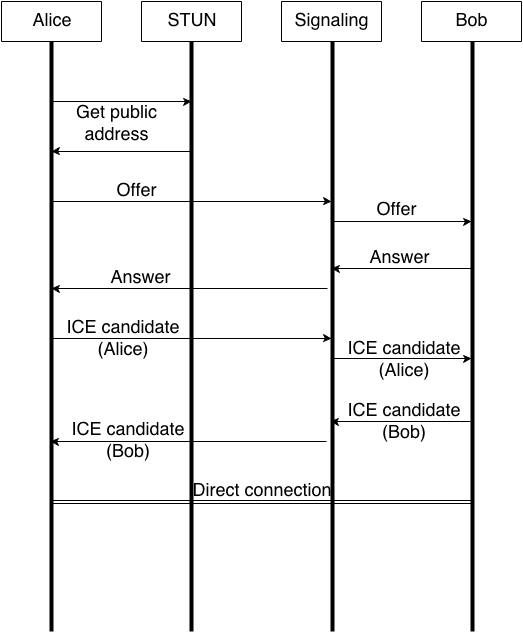
\includegraphics[width=9cm]{Images/WebRTC}
    \caption{Examplary WebRTC connection}
    \label{fig:webrtc}
\end{figure}


\section{Massive Collaborative Editing}

One application for a gossip-based WebRTC network is a massive collaborative editor \cite{nedelec:hal-00921633}\cite{MassCollab} that runs in the web browser.
Unlike current solutions such as Google Docs, Microsoft Word Online or Etherpad we want to support millions of users on one document (e.g. Google Docs only allows 50 users to work on one document).
\cite{MassCollab} describes how parallel editing can scale well with the number of users, implied that some sort of broadcast exists.
However, no assumptions are made about how this broadcast is done.
A centralized service or a fully connected graph do not scale well with the user count.
Instead, using the proposed gossip-based peer-to-peer protocol for WebRTC will make the application more scalable and robust.

%-------------------------------------------------------------------------------------------------------------

% \part{State-of-the-Art} % Comment it out if the state-of-the-art requires several chapters.
                          % Most often, you'll then have a presentation chapter followed by a critical synthesis chapter.
                          % In that case, you must commen tour your work part, hereafter.
% \label{part:StateOfTheArt}

\chapter{State of the Art}
\label{chap:StateOfTheArt}

This chapter introduces fundamental algorithms and concepts. 

\section{Gossip Protocol}

Gossip, also refered to as \emph{epidemic dissemination}, is a  communication protocol initially inspired by observing of how gossips spread in social networks or how diseases spread over a population.
It trades reliability guarantees against scalability properties \cite{Eugster:2003:LPB:945506.945507} and it has been applied to various large scale systems, with the purpose of information dissemination \cite{Demers:1987:EAR:41840.41841}, information aggregation \cite{Jelasity:2005:GAL:1082469.1082470}, network management \cite{conf/dsom/VoulgarisS03} and many more.

The basic idea behind gossip works as follows:
a network is a graph $G=(V,E)$ where $V=\{1,...,n\}$ is a set of $n$ nodes.
Let $E \subset V \times V$ denote neighboring\footnote{In this paper, nodes are considered neighbors if they are directly connected to each other} nodes and let $d_i$ denote the degree of node $i$ in $G$ where 
$d_i$ is constrained by the configuration parameter $c \in \mathbb{Z}_{>0}$ which is called Fanout.
The Fanout defines the number of nodes that are selected when a message is broadcast from a node.
A high value generates a lot of redundant messages while being more fault tolerant and reliable. 
$V$ and $E$ constantly change as nodes leave and join the network and nodes update there neighbors to maintain a uniform distribution.

Assuming a node $i$ wants to broadcast a message $m$ - It sends $m$ to its $d_i$ neighboring nodes. 
A receiving node $j$ evaluates if it already knows $m$ \cite{Koldehofe03buffermanagement} - and if not, it will repeat the previous procedure: broadcast to its $d_j$ neighboring nodes and so forth. 
Usually three types of epidemic dissemination of messages can be distinguished:
\begin{itemize}
    \item \textbf{Push:} When receiving a message, a node sends it to all other nodes in its view.
    \item \textbf{Pull:} A node periodically queries one random other node to check for messages it has not received yet.
    \item \textbf{Push-Pull:} A node sends a message to another random peer and, additionally, queries said peer for data.
\end{itemize}

When $n$ is very large, for a given node $i$ it applies that $d_i << n$.
This is necessary for scalability reasons as, otherwise, the list of neighbors might exhaust a nodes memory and maintaining the list in presence of churn\footnote{Nodes constantly join and leave the network} would be too expansive.
We will call $\mathcal{N}_i \equiv \{j\in V:(i,j)\in E\}$ the \textbf{partial view} of $i$.
The partial view should consist of a random sample of $V$.

\section{Peer Sampling Service}

The peer sampling service \cite{Jelasity:2004:PSS:1045658.1045666}, or, random peer sampling (RPS), is a membership protocol.
The purpose of RPS is to provide each peer with a \emph{uniform sample} of $V$ in a distributed and scalable manner.
It can be used in a variety of gossip-based protocols, for example in topology management \cite{Jelasity:2009:TGF:1570533.1570626}. 
The peer sampling service consists of a simple API:

\begin{itemize}
    \item{\textbf{init:}} Initializes the service on a given node if this has not been done before. This is implementation dependent.
    \item{\textbf{getPeer:}} Returns a peer address if the network contains more than one node. The returned address is a sample drawn from the group. This method can also be used to return multiple random peers, either by providing a paramter $n$ to the function or by simply calling the method multiple times.
\end{itemize}

There are two strategies to maintain partial views in peer sampling services \cite{Leitao_gossip-basedbroadcast} that will play an important role in our evaluation:

\begin{itemize}
    \item{\textbf{Reactive:} The partial view only changes when $V$ changes (Nodes join or leave) and remains stable otherwise.
An example algorithm is SCAMP \cite{Ganesh:2001:SPL:648089.747488}.}
    \item{\textbf{Cyclic:} The partial view is periodically updated every $\bigtriangleup T$ time units and membership information are exchanged with neighbors.
An example algorithm is CYCLON \cite{Voulgaris05cyclon:inexpensive}.}
\end{itemize}

\section{Newscast}

The newscast protocol \cite{Voulgaris03arobust}\cite{Jelasity02large-scalenewscast} serves as information dissemination protocol where joining and leaving the network is very cheap.
If a node wants to join the system it only needs to know the address of an arbitrary member, for leaving the network no action is necessary, the node can simply stop communicating.

Abstractly it works by employing a \emph{news agency}.
All peers must implement a simple API consisting of \textbf{getNews()} and \textbf{newsUpdate(news)}.
For the protocol, peers are passive and are queried by the news agency.
\textbf{getNews} is called regularly by the agency to obtain any news. 
Additional to that, the news agency provides the whole collective with news by calling \textbf{updateNews}.
The news agency can be implemented in a fully distributed fashion by running an associated \emph{correspondent} that runs on the same machine as the peer \cite{Voulgaris03arobust}.
Each correspondent has a news cache of size $c$ where the news optained from the peer are timestamped and stored.
Every $\bigtriangleup T$ (\textit{refresh interval}) time the correspondents exchange their caches applying the following steps\footnote{as described in \cite{Voulgaris03arobust} Section 2.1}:

\begin{enumerate}
    \item{Request a fresh news item from the local peer by calling \textbf{getNews}. Add the item to the cache.}
    \item{Radomly select a peer correspondent by considering the netwok address of other (and available) correspondents as found in the cache.}
    \item{Send all cache entries to the selected peer, and, in turn, receive all the peer's cache entries. Merge the received entries into the local cache.}
    \item{Pass the received cache entries from the peer node to the local peer by calling \textbf{newsUpdate}.}
    \item{The correspondent now has $2c$ cache entries; it subsequently throws away the $c$ oldest ones.}
\end{enumerate}

The receiving correspondent executes the last three steps as well.
Synoptical, each node knows only a small, permanently changing set of peers of which one is chosen to exchange information.

\begin{algorithm}
    \caption{Active}
    \begin{algorithmic}[1]
        \State // Executed by any correspondent    
        \While{Termination condition not reached}
            \State wait $\bigtriangleup T$
            \State $news \gets$ getNews()
            \State $cache \gets cache \cup \{news\}$
            \State $peer \gets$ selectRadom( getAddresses($cache$))
            \State send $cache$ to $peer$
            \State $otherCache \gets$ receive from $peer$
            \State $cache \gets$ merge($cache$, $otherCache$)
            \State newsUpdate($otherCache$)
            \State
            \State // potentially expensive with handshake, as we need to establish connections
            \State $cache \gets$ first(orderByAge($cache$), $c$)
        \EndWhile
    \end{algorithmic}
\end{algorithm}

\begin{algorithm}
    \caption{Passive}
    \begin{algorithmic}[1]
        \State // Listens on any correspondent
        \Procedure{OnExchange}{$peer$, $otherCache$}
        \State send $cache$ to $peer$
        \State $cache \gets$ merge($cache$, $otherCache$)
        \State newsUpdate($otherCache$)
        \State $cache \gets$ first(orderByAge($cache$), $c$)
        \EndProcedure
    \end{algorithmic}
\end{algorithm}

\section{SCAMP}

The probabilistic scalable membership protocol (SCAMP)\cite{Ganesh:2001:SPL:648089.747488} is a reactive peer sampling service.
The size of its local views adapt automatically to a desired value of $(c+1)\log{n}$ where $c$ is a  parameter which specifies the degree of robustness to failure(\cite{Kermarrec:2003:PRD:766617.766623}, \emph{Theorem 1}).
It maintains two separated partial views\cite{Ganesh:2003:PMM:642778.642782}, one for receiving gossip messages (InView $\mathcal{N}^{in}$), one for sending gossip messages (PartialView $\mathcal{N}^{out}$).

If a new node $k$ wants to join the network $G(V,E)$ it needs to have one member $i \in V$ in $\mathcal{N}_k^{out}$ and send a subscription request to $i$.
On receiving a subscription request, $i$ forwards the new peer to all members of its own $\mathcal{N}_i^{out}$, and, additianally, creates $c$ copies of the new subscription and forwards them to randomly chosen nodes in $\mathcal{N}_i^{out}$.
On receiving a fowarded subscription for node $k$, a receiving node $j$ integrates $k$ into its $\mathcal{N}_j^{out}$ with probability $p$ which depends on the size of $\mathcal{N}_j^{out}$ ($p_i=\frac{1}{1+|\mathcal{N}_i^{out}|}$). 
If $j$ does not integrate $k$, it forwards it to another randomly chosen peer from its $\mathcal{N}_j^{out}$.
When a node $i$ decides to keep the subscription of a node $j$, it integrates $j$ into its $\mathcal{N}_i^{out}$ and notifies $j$ to put $i$ into its $InView_j$.
On leaving the network, the leaving node $j$ sends a \emph{replace request} containing a peer from its $\mathcal{N}_j^{out}$ to $|\mathcal{N}_j^{in}|-c$ peers in its $\mathcal{N}_j^{in}$ and a \emph{deleting request} to the remaining ones.
When a node $i$ receives the \emph{replace request} from $j$, it will replace $j$ for the sent peer in its $\mathcal{N}_i^{out}$.

A subscription has a finite lifetime called \emph{lease}\footnote{The lease is implementation dependend: it could be set individually or it could be set globally}.
When expired, the subscribed node will be removed from all PartialViews.
It is a nodes responsibility to resubscribe once its subscription expires.
This mechanic ensures that failed nodes will not remain in the network.
Furthermore, the lease mechanism rebalances the network making it more robust.
Indeed, when a peer joins the system, it only has one node in its partial view, which makes it vulnerable to failures.
However, when peers resubscribe, it adds the link to its inView and therefore, to others partial view.
Hence, even the new peers can get subscription requests.

Pseudocode: \cite{Ganesh:2001:SPL:648089.747488}, Section 2.1
\begin{algorithm}
    \caption{Subscription management}
    \begin{algorithmic}[1]
        \Procedure{OnSubscribe}{$subscriber$}
        \For{each $peer$ in $\mathcal{N}^{out}$}
        \State send \textbf{forwardedSubscription} with $subscriber$ to $peer$
        \EndFor
        \For{each $peer$ in sample($\mathcal{N}^{out}$, $c$)}
        \State send \textbf{forwardedSubscription} with $subscriber$ to $peer$
        \EndFor
        \EndProcedure
    \end{algorithmic}
\end{algorithm}

\begin{algorithm}
    \caption{Handling of a forwarded subscription}
    \begin{algorithmic}[1]
        \Procedure{OnForwardedSubscription}{$subscriber$}
        \State $keep \gets$ randomChoiceBetween0and1()
        \State $keep \gets \lfloor (|\mathcal{N}^{out}| + 1) * keep \rfloor$
        \If{$keep \equiv 0 $ and $subscriber \notin \mathcal{N}^{out}$}
        \State 
        \State // potentially very expensive as the handshake must be traced over
        \State // possibly many hops
        \State $\mathcal{N}^{out} \gets \mathcal{N}^{out} \cup \{subscriber\}$
        \State
        \Else
        \State $peer \gets$ sample($\mathcal{N}^{out}$, $1$)
        \State send \textbf{forwardSubscription} with $subscriber$ to $peer$
        \EndIf
        \EndProcedure
    \end{algorithmic}
\end{algorithm}

\section{CYCLON}

CYCLON \cite{Voulgaris05cyclon:inexpensive} is a cyclic peer sampling service.
Each peer maintains a partial view of size $c$ and repeatedly exchanges its view with a neighbor - this operation is called a shuffle.
The protocol works as follows\footnote{Enhanced Shuffling, described in \cite{Voulgaris05cyclon:inexpensive}}:

Every $\bigtriangleup T$ time unit a node $i$ executes the shuffle function:

\begin{enumerate}
    \item{Increase by one the age of all neighbors.}
    \item{Select neigbor $j$ with the highest age among all neighbors, and $l-1$\footnote{$1 \le l \le c$}} other random neighbors.
    \item{Replace $j$'s entry with a new enty of age 0 and with $i$'s address.}
    \item{Send the updated subset to peer $j$}
    \item{Receive from $j$ a subset of no more than $t$ of its own entries.}
    \item{Discard entries pointing at $j$ and entries already contained in $i$'s partial view.}
    \item{Update $i$'s partial view to include all remaining entries, by firstly using empty slots (if any), and secondly replacing entries among the ones sent to $j$}
\end{enumerate}

On receiving the shuffle request from $i$ at $j$, $j$ sends back a random subset of $l$ of its neighbors and updates its own partial view with the sent data but it does not increase the age of the items in the partial view.
When a node $i$ does not get a response from a node $j$ after it sent a shuffle request it will discard node $j$ from its partial view as it seems to be failed. 
Because of this, failed nodes will be removed from the network in bounded time.
As in SCAMP and newscast, if a node wants to join the network, it needs to know another node that is already part of it.

\begin{algorithm}
    \caption{Active}
    \begin{algorithmic}[1]
        \While{Termination condition not reached}
        \State wait $\bigtriangleup T$
        \State $partialView \gets$ increaseAge($partialView$)
        \State $peer \gets$ max(orderByAge($partialView$))
        \State $rand \gets $ sample($partialView \backslash \{peer\}$ , $l-1$) $\cup \{$[addr:$ownAddress$, age:$0$]$\}$
        \State send $rand$ to $peer$
        \State $otherRand \gets $ receive from $peer$
        \State $otherRand \gets otherRand \backslash \{partialView \cup \{[addr:ownAddress, age:*]\}\}$
        \State $partialView \gets partialView \backslash rand$
        \State
        \State // this part is very expensive with handshake
        \State $partialView \gets partialView \cup otherRand$
        \State
        \While{$|partialView| < c$}
        \State $partialView \gets shift(orderByAge(rand))$ // shift removes the first element of an list
        \EndWhile
        \EndWhile
    \end{algorithmic}
\end{algorithm}

\begin{algorithm}
    \caption{Passive}
    \begin{algorithmic}[1]
        \Procedure{OnExchange}{$peer$, $otherRand$}
        \State $rand \gets$ sample($partialView$, $l$)
        \State send $rand$ to $peer$
        \State $otherRand \gets otherRand \backslash partialView$
        \State $partialView \gets partialView \backslash rand$
        \State
        \State // this part is very expensive with handshake
        \State $partialView \gets partialView \cup otherRand$
        \State
        \While{$|partialView| < c$}
        \State $partialView \gets shift(orderByAge(rand))$ // shift removes the first element of an list
        \EndWhile
        \EndProcedure
    \end{algorithmic}
\end{algorithm}

%\section{Synthesis}

%\begin{table*} % Use the starred version if the table is too large for a two-column document (screen version)
%    \begin{center}
%        \begin{tabular}{c|ccccc}
%                         & Proposal 1 & \ldots & Proposal $i$ & \ldots & Proposal $n$ \\
%            \hline
%            Criteria $1$ & $\surd$    &        &              &        & $\surd$      \\
%            \ldots       & \ldots     & \ldots & \ldots       & \ldots & \ldots       \\
%            Criteria $j$ & $\approx$  &        &              &        &              \\
%            \ldots       & \ldots     & \ldots & \ldots       & \ldots & \ldots       \\
%            Criteria $m$ &            &        & $\surd$      &        &              \\
%        \end{tabular}
%    \end{center}
%    \caption{Comparison of various proposals}
%    \label{tab:ProposalsComparison}
%\end{table*}

\section{Conclusion}

All of the mentioned algorithms have certain problems and limitations when handshaking is added.
In newscast the value of $\bigtriangleup T$ must be higher than the time the peers need to connect.
This could be implemented by setting $CONNECTION-TIMEOUT < \bigtriangleup T$.
This will, possibly significantly, increase the time a news will take to be fully disseminated into the network.

SCAMP will face the need for a much more complex algorithm as it needs to provide a routed signalling service over possibly many nodes.
A way to repair a route in case of node-failure must be found as SCAMP would otherwise be extremly unstable.

CYCLON faces similar issues as newscast and can, accordingly, be modified to fullfill the basic needs for handshaking (set $\bigtriangleup T$ higher than the connection timeout).
The problem here is the same as in newscast: messages will be dissemiated slower.

%--------------------------------------------------------------------------------

% \part{Proposals} % Commet it out if this has been done for the state-of-the-art
% \label{part:Proposals}

\chapter{Proposals}
\label{chap:Proposals}

\section{General Approach}

Our research question states: \emph{What is the cheapest handshake gossip algorithm?}
We consider an algorithm to be cheaper than another, if, on average, it employs less handshakes.
This also counts the number of peers in an \emph{intermediate handshake}.
We consider a handshake to be \emph{intermediate} if a peer $i$ cannot directly hoist a connection between two nodes $a$ and $b$ but instead needs to apply $m, m < 0$ intermediate nodes to establish a connection.
This is neccessary due to the requirement to reduce the connections to a centralized signaling server as much as possible and, instead, use the decentralized peer-to-peer network to carry out the signalling service, as soon as a node is member of the system.

In a first step we use PeerSim\cite{Montresor_peersim:a} to evaluate the number of handshakes within the well-known algorithms.
To do so, we need to adapt the algorithms accordingly.
The algorithm that provides the best results will be implemented with WebRTC.

The next step is the proposal of an improved algorithm that directly addresses the need for handshaking.
Again, this algorithm is implemented in WebRTC and tested against the best algorithm from the PeerSim-evaluation.
This tests are run on the Grid'5000 testbed using CREATE\cite{MassCollab} as a base implementation.

\begin{figure}[!]
   \centering
   \setlength{\unitlength}{5cm}
   \begin{picture}(1.2, 1.3)
     \put(0, 0){\vector(1, 0){1.15}}
     \put(1.17, -.015){$n$}
     \put(0, 0){\vector(0, 1){1.15}}
     \put(0, 1.19){\makebox(0, 0){$Handshakes$}}
     \qbezier(0.0,0.0)(0.4128,0.0)(0.7218,0.618)
     \qbezier(0.0,0.0)(0.4306,0.0)(0.7703,0.5662)
     \qbezier(0.0,0.0)(0.4436,0.0)(0.8081,0.5207)
     \qbezier(0.0,0.0)(0.4758,0.0)(0.9102,0.362)
     \put(1, -.02){\line(0, 1){.04}}
     \put(1, .06){\makebox(0, 0){$100.000$}}
     \put(-.02, 1){\line(1, 0){.04}}
     \put(.03, .98){$100.00$}
   \end{picture}
   \caption{Numbers of handshakes established by the signaling server}
\end{figure}

\begin{figure}[!]
   \centering
   \setlength{\unitlength}{5cm}
   \begin{picture}(1.2, 1.3)
     \put(0, 0){\vector(1, 0){1.15}}
     \put(1.17, -.015){$n$}
     \put(0, 0){\vector(0, 1){1.15}}
     \put(0, 1.19){\makebox(0, 0){$Handshakes$}}
     \qbezier(0.0,0.0)(0.4128,0.0)(0.7218,0.618)
     \qbezier(0.0,0.0)(0.4306,0.0)(0.7703,0.5662)
     \qbezier(0.0,0.0)(0.4436,0.0)(0.8081,0.5207)
     \qbezier(0.0,0.0)(0.4758,0.0)(0.9102,0.362)
     \put(1, -.02){\line(0, 1){.04}}
     \put(1, .06){\makebox(0, 0){$100.000$}}
     \put(-.02, 1){\line(1, 0){.04}}
     \put(.03, .98){$100.00$}
   \end{picture}
   \caption{Numbers of handshakes established by the signaling service inside the peer-to-peer network}
\end{figure}

\section{Proposal 1}

TBD
%For each of contribution, it is advisable:
%\begin{itemize}
%   \item to introduce it thanks to preliminary intuitive ideas (coming both from your understanding of the problem and from the ideas brought to you by the literature);
%   \item then to formalise them trough mathematical models and/or algorithms;
%   \item then demonstrated, as much as possible;
%   \item finally analysed (e.g., Do you solve the whole problem? Is the solution resource efficient? Etc.).
%\end{itemize}

\section{Proposal 1}

Etc.

\section{Conclusion}

%If too many ideas have been enumerated and none can be totally and formally demonstrated to be the best, then some choice has probably to be made in order to limit the time-consuming experiments that follow.  It is preferable to achieve a few well-conducted experiments that will provide unquestionable conclusions though in a limited scope.
TBD

%--------------------------------------------------------------------------------

%\part{Experiments and Results} % in case of several chapters, then name the chapters differently
%\label{part:Experiments}

\chapter{Experiments and Results}
\label{chap:Experiments}

%When it is not possible to work only at the theoretical level, experiments will take place.  In Computer Science, this is most often through developing code then running experiments with it and analysing the output.

%Notice that if both parts are important, or if more than one proposal has been investigated, it is certainly better to split this chapter into several distinct chapters.  In the former case, you can even enclose these chapters inside a new part.
TBD

\section{Experiment 1}

%Be extremely precise when describing your experiments.  They must be reproducible by any reader deeply interested in your work.

%You should describe all the hypotheses and constraints related to the manipulated data and the developed algorithms or used softwares.  Check them carefully in order not to draw false conclusion from bad inputs or erroneous processing!

%\begin{figure}
%   \centering
%   \setlength{\unitlength}{5cm}
%   \begin{picture}(1.2, 1.3)
%     \put(0, 0){\vector(1, 0){1.15}}
%     \put(1.17, -.015){$x$}
%     \put(0, 0){\vector(0, 1){1.15}}
%     \put(0, 1.19){\makebox(0, 0){$y$}}
     % qbezier P1=(0.0/0.0) m1=0.0
     %         P2=(0.2998/0.905) m2=10.0
%     \qbezier(0.0,0.0)(0.2093,0.0)(0.2998,0.905)
     % qbezier P1=(0.0/0.0) m1=0.0
     %         P2=(0.4625/0.8198) m2=5.0
%     \qbezier(0.0,0.0)(0.2985,0.0)(0.4625,0.8198)
     % qbezier P1=(0.0/0.0) m1=0.0
     %         P2=(0.5757/0.744) m2=3.3333
%     \qbezier(0.0,0.0)(0.3525,0.0)(0.5757,0.744)
     % qbezier P1=(0.0/0.0) m1=0.0
     %         P2=(0.6589/0.677) m2=2.5
%     \qbezier(0.0,0.0)(0.3881,0.0)(0.6589,0.677)
     % qbezier P1=(0.0/0.0) m1=0.0
     %         P2=(0.7218/0.618) m2=2.0
%     \qbezier(0.0,0.0)(0.4128,0.0)(0.7218,0.618)
     % qbezier P1=(0.0/0.0) m1=0.0
     %         P2=(0.7703/0.5662) m2=1.6667
%     \qbezier(0.0,0.0)(0.4306,0.0)(0.7703,0.5662)
     % qbezier P1=(0.0/0.0) m1=0.0
     %         P2=(0.8081/0.5207) m2=1.4286
%     \qbezier(0.0,0.0)(0.4436,0.0)(0.8081,0.5207)
     % qbezier P1=(0.0/0.0) m1=0.0
     %         P2=(0.8381/0.4806) m2=1.25
%     \qbezier(0.0,0.0)(0.4536,0.0)(0.8381,0.4806)
     % qbezier P1=(0.0/0.0) m1=0.0
     %         P2=(0.862/0.4454) m2=1.1111
%     \qbezier(0.0,0.0)(0.4611,0.0)(0.862,0.4454)
     % qbezier P1=(0.0/0.0) m1=0.0
     %         P2=(0.8814/0.4142) m2=1.0
%     \qbezier(0.0,0.0)(0.4672,0.0)(0.8814,0.4142)
     % qbezier P1=(0.0/0.0) m1=0.0
     %         P2=(0.8972/0.3866) m2=0.9091
%     \qbezier(0.0,0.0)(0.4719,0.0)(0.8972,0.3866)
     % qbezier P1=(0.0/0.0) m1=0.0
     %         P2=(0.9102/0.362) m2=0.8333
%     \qbezier(0.0,0.0)(0.4758,0.0)(0.9102,0.362)
%     \put(0.5757, 0.744){\circle*{.015}}
%     \put(0.6,    0.74){$(u,v)$}
%     \put(0.5,    0.05){$L$}
%     \put(0.18,    0.45){$L$}
%     \put(1, -.02){\line(0, 1){.04}}
%     \put(1, .06){\makebox(0, 0){$L$}}
%     \put(-.02, 1){\line(1, 0){.04}}
%     \put(.03, .98){$L$}
%   \end{picture}
%   \caption[Quality of the results obtained]
%           {Quality of the results obtained [Source : << \emph{Graphics in LaTeX 2$_\varepsilon$} >>, page~23]}
%   \label{fig:Courbes}
%\end{figure}

%In this part of the report, you should put forth \emph{synthetic results}, in the form of several tables and figures (e.g., See figure~\ref{fig:Courbes}%
%\footnote{Urs Oswald, \emph{``Graphics in LaTeX 2$_\varepsilon$,''} March 2003, \url{http://www.ursoswald.ch}.}%
%)

%For the sake of completeness, these synthetic results must be supported by the base results from which they are derived.  These lengthy results have to be put into the appendices (e.g., See Appendix~\ref{app:Measures}).
TBD

\section{Experiment 2}

Etc.

\section{Conclusion}

%The conclusion of this chapter (alternatively of this part) is normally the culmination of this research work.  All the quality of the work, along with its limitations, have to be emphasised.  Also, you can draw some personal conclusion on the way this study has been conducted and what could be done better should you have the chance to restart it anew.
TBD

%--------------------------------------------------------------------------------

\chapter{Conclusion}

%By the end of the work, you should firstly summarise the main steps and key results of the study.  Then, you should describe the research directions that this work opens, both simple extensions and new endeavours.
TPD

\section{Summary}

%Even if it is yet another repetition, it is convenient to summarise not the whole report but at least your own work and results, stressing their value.
TBD

\section{Outcomes}

%The most valuable teachings of the work (there always have) must be emphasised.  Some can be personal.
TBD

\section{Research directions}

%It is quite rare that a given work totally closes a topic!  Even in that case, it remains possible to introduce new research directions, more or less connected to the topic and the new state-of-the-art.  More generally, you can mention all and every question that has arisen during the course of your work.
TBD

%--------------------------------------------------------------------------------

\bibliography{report}

\listoffigures{}

\listoftables{}

\listofalgorithms{}

\appendix


\chapter{Reminder}
\label{app:Reminder}

%A reminder appendix can contain information that is supposed to be known by the reader but that is worth to include in the report in order to make it self-contained.

%If the reminder contains only a list of short definitions, consider naming it ``Glossary'' instead.  You can have both.

%For instance, we can write down: ``The average can be computed differently whether the individuals are grouped or not, their exact number known or only their frequency, i.e.:
%\begin{eqnarray}
%    \mu & = & \frac{1}{n} \sum_{i=1}^n x_i\\
%    \mu & = & \frac{1}{N} \sum_{i=1}^m x_i \times n_i\\
%    \mu & = & \sum_{i=1}^m x_i \times f_i
%\end{eqnarray}
%with:
%\begin{itemize}
%    \item $N = \sum_{i=1}^m n_i$ ;
%    \item $f_i = \frac{n_i}{N}$.''
%\end{itemize}
TBD


\chapter{Detailed Measures}
\label{app:Measures}

%Lengthy sub-results have to be put in appendices.  In other words, too boring details should be postponed to the very last part of the reading, that is when the reader is interested enough in understanding the very details of your proposal, especially if he or she intend to reproduce your experiment.  This is also true for detailed algorithms, etc.

%This (these) appendix(ces) is (are) mandatory in order for the report to contain of the ``proofs'' of its claims, i.e., to really provide a \emph{scientific} work.
TBD

\chapter{Annotated References}
\label{app:FichesLecture}

%It is a good idea to provide a short summary of each of the papers in the references.
%For each paper or book (in rare cases a \emph{complete and persistent} web site), you should extract the following kind of information:  firstly, a short summary;  then, your own analysis.

%This is slightly redundant with the state-of-the-art chapter. However, notice that it lacks the overall synthesis, and it focuses on a single paper at a time.  In fact, this greatly helps to achieve the state-of-the-art.
TBD

\paragraph{\emph{Title of a paper}.}

TBD
%Describe rapidly what problem is attacked in the paper (add the reference, e.g. \cite{Pascal-1671}).

\subparagraph{Summary.}

TBD
%The summary presents the main idea of the paper and the work conducted \emph{by the authors} up to their conclusions.

\subparagraph{Analysis.}

%It is only during a second phase that you can analyse the contents of the paper, i.e., verify it (errors are always possible in the scientific literature!), express your opinion about the advances claimed by the paper, and establish a connection with your own work.
TBD

\paragraph{\emph{Title of a paper}.}

Etc.

\chapter{Schedule}

This appendix is \emph{mandatory}.

Figure~\ref{fig:Drafting} shows the draft schedule establish \emph{a priori}\ldots

\begin{figure*}
% - Use the starred version in order to put floats on two columns
% - Possibly, use the "\ifscreen ... \else ... \fi"" alternative to orientate correctly
%   the planning with respect to the orientation of the paper (cf. below for the auto-evaluation)
   \centering
      \emph{<Insert a Gantt's diagram.>}
   \caption{Drafting}
   \label{fig:Drafting}
\end{figure*}

Figure~\ref{fig:Planning} introduce the planning that has been build week after week during the course of the work.

\begin{figure*}
   \centering
         %\rotatebox{90}{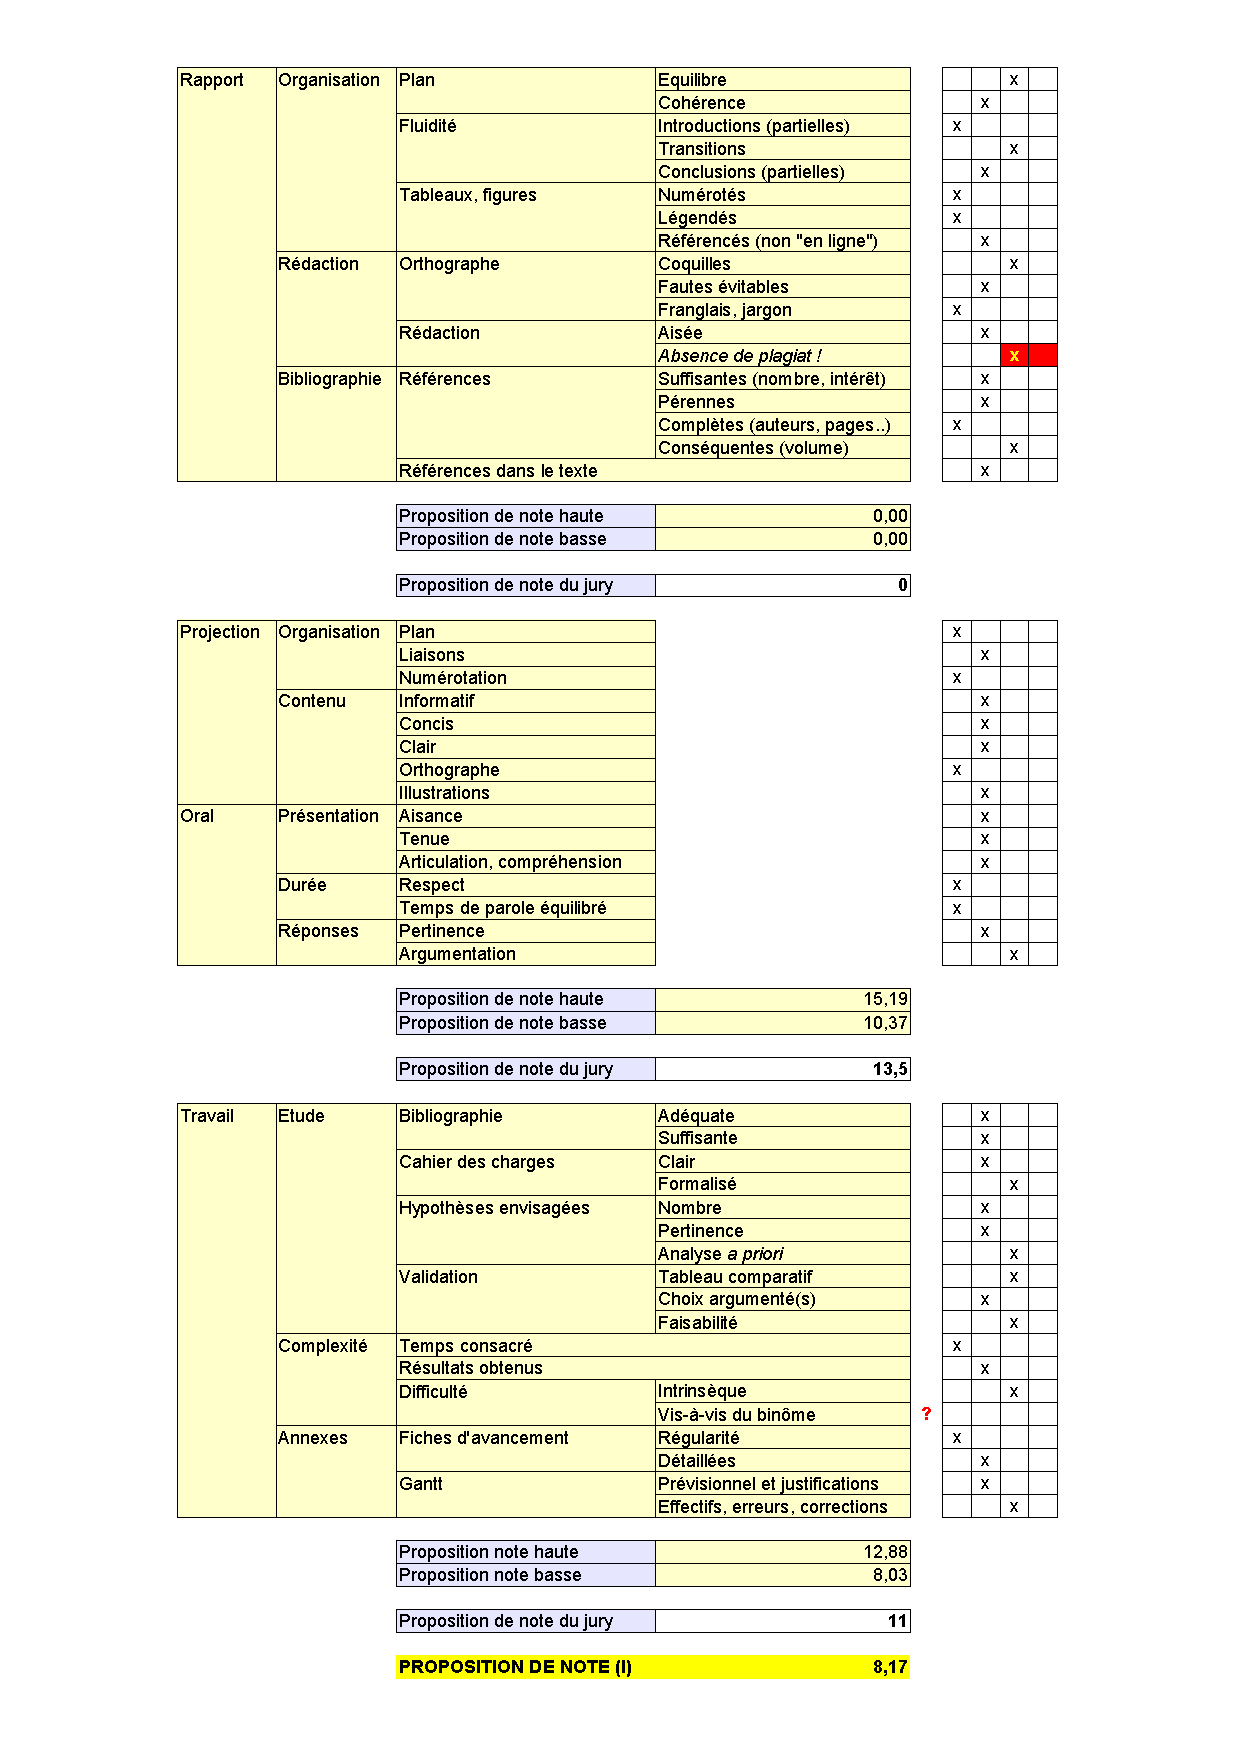
\includegraphics[width=0.9\textheight]{Images/Grille-Evaluation-PRD1}}
   \rotatebox{270}{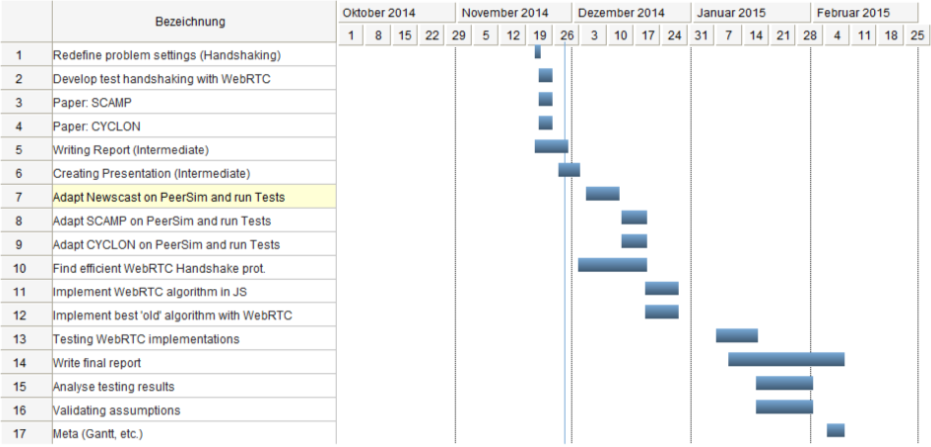
\includegraphics[width=22cm]{Images/gantt}}
   \caption{Planning}
   \label{fig:Planning}
\end{figure*}

Discuss differences between the drafting and the planning as well as lessons learned on the management of a research project or R\&D project.

\chapter{Weekly Reports}
\label{ann:WeeklyReports}

This appendix is \emph{mandatory}.

\begin{fichesuivi}{September 29, 2014}{October 04, 2014}
   \tempstravailA{6}{00}
   \tempstravailB{0}{00}

   \begin{travaileffectue}
      \begin{itemize}
          \item Studying paper \emph{LSEQ: an Adaptive Structure for Sequences in Distributed Collaborative Editing}
         \item Studying paper T-Man: Gossip-based Overlay Topology Management
      \end{itemize}
   \end{travaileffectue}

   %\begin{travailnoneffectue}
   %   \begin{itemize}
   %      \item Task 1:  reasons; postponements, cancellations; etc.;
   %   \end{itemize}
   %\end{travailnoneffectue}

   %\begin{echange}
   %   \begin{itemize}
   %      \item Questions;
   %      \item Answers;
   %      \item Clarification, comprehension;
   %      \item Choices, orientations, reorientations;
   %      \item Etc.
   %   \end{itemize}
   %\end{echange}

   \begin{planification}
      \begin{itemize}
         \item Researches to be conducted
      \end{itemize}
   \end{planification}
\end{fichesuivi}

\begin{fichesuivi}{October 06, 2014}{October 10, 2014}
   \tempstravailA{8}{30}
   \tempstravailB{0}{00}

   \begin{travaileffectue}
      \begin{itemize}
          \item {Paper: The Peer Sampling Service: Experimental Evaluation of Unstructured Gossip-Based Implementations}
        \item {Paper: Gossip-based broadcast protocols}
        \item {Technical evaluation: WebRTC}
        \item {Technical evaluation: PeerJS}
      \end{itemize}
   \end{travaileffectue}

   \begin{travailnoneffectue}
   \end{travailnoneffectue}

   \begin{echange}
   \end{echange}

   \begin{planification}
      \begin{itemize}
         \item Researches to be conducted
        \item Testimplementations with WebRTC 
     \end{itemize}
   \end{planification}
\end{fichesuivi}

\begin{fichesuivi}{October 13, 2014}{October 18, 2014}
   \tempstravailA{17}{00}
   \tempstravailB{0}{0}

   \begin{travaileffectue}
      \begin{itemize}
   \item {Testing PeerJs -> Implementation of Chat prototype}
   \item {Papers: Detecting Causal Relationships in Distributed Computations: In Search of the Holy Grail}
     \end{itemize}
   \end{travaileffectue}

   \begin{travailnoneffectue}
   \end{travailnoneffectue}

   \begin{echange}
   \end{echange}

   \begin{planification}
      \begin{itemize}
   \item {prototype for Peer-Samping-Service}
   \item {prototype for T-Man}
     \end{itemize}
   \end{planification}
\end{fichesuivi}

\begin{fichesuivi}{October 20, 204}{October 25, 2014}
   \tempstravailA{22}{30}
   \tempstravailB{0}{00}

   \begin{travaileffectue}
      \begin{itemize}
          \item {Implementing prototype for Peer-Samping-Service (RSP) based on PeerJS}
   \item {Paper: A Robust and Scalable Peer-to-Peer Gossiping Protocol}
   \item {Paper: SCAMP: Peer-to-peer lightweight membership service for large-scale group communication}
   \item{Buffer Management in Probabilistic Peer-to-Peer Communication Protocols}
     \end{itemize}
   \end{travaileffectue}

   \begin{travailnoneffectue}
       \begin{itemize}
           \item{Prototype for T-Man: Implementation of RSP took longer than expected. }
        \end{itemize}
   \end{travailnoneffectue}

   \begin{echange}
   \end{echange}

   \begin{planification}
      \begin{itemize}
   \item {prototype for T-Man}
     \end{itemize}
   \end{planification}
\end{fichesuivi}

\begin{fichesuivi}{October 27, 2014}{01 November, 2014}
    \tempstravailA{6}{00}
   \tempstravailB{0}{00}

   \begin{travaileffectue}
      \begin{itemize}
          \item {Implementation of T-Man with PeerJS (needs RPS)}
     \end{itemize}
   \end{travaileffectue}

   \begin{travailnoneffectue}
      \begin{itemize}
          \item {still some problems with RPS (create new unit tests)}
     \end{itemize}
   \end{travailnoneffectue}

   \begin{echange}
   \end{echange}

   \begin{planification}
      \begin{itemize}
         \item Researches to be conducted
   \item {testing prototype for T-Man}
     \end{itemize}
   \end{planification}
\end{fichesuivi}

\begin{fichesuivi}{November 03, 2014}{November 06, 2014}
   \tempstravailA{14}{00}
   \tempstravailB{00}{00}

   \begin{travaileffectue}
      \begin{itemize}
          \item {Paper: CYCLON: Inexpensive Membership Management for Unstructured P2P Overlays}
          \item {Test: Implementation of T-Man with PeerJS (needs RPS)}
     \end{itemize}
   \end{travaileffectue}

   \begin{travailnoneffectue}
   \end{travailnoneffectue}

   \begin{echange}
   \end{echange}

   \begin{planification}
      \begin{itemize}
         \item Researches to be conducted
     \end{itemize}
   \end{planification}
\end{fichesuivi}

\begin{fichesuivi}{November 10, 2014}{November 15, 2014}
   \tempstravailA{20}{00}
   \tempstravailB{0}{00}

   \begin{travaileffectue}
      \begin{itemize}
        \item {Paper: Lightweight Probabilistic Broadcast}
        \item {Start writing report: "A Scalable Network Topology for Massive Collaborative Editing"}
    \end{itemize}
   \end{travaileffectue}

   \begin{travailnoneffectue}
   \end{travailnoneffectue}

   \begin{echange}
   \end{echange}

   \begin{planification}
      \begin{itemize}
         \item Start with a draft of the report
         \item Researches to be conducted
      \end{itemize}
   \end{planification}
\end{fichesuivi}

\begin{fichesuivi}{November 17, 2014}{November 22, 2014}
    \tempstravailA{30}{30}
   \tempstravailB{0}{00}

   \begin{travaileffectue}
      \begin{itemize}
   \item {Write Introduction of Paper: "Topology Management for Massive Collaborative Editing"}
      \end{itemize}
   \end{travaileffectue}

      \begin{itemize}
          \item {Change the reasearch topic: We figured that some fundamental issues MUST be addressed before the old topic (Topology Management). New Topic: Handshaking gossiping, as this is essential for the implementation.}
      \end{itemize}
   \begin{travailnoneffectue}
   \end{travailnoneffectue}

   \begin{echange}
   \end{echange}

   \begin{planification}
      \begin{itemize}
         \item Write the report
      \end{itemize}
   \end{planification}
\end{fichesuivi}

\begin{fichesuivi}{}{}
   \tempstravailA{30}{30}
   \tempstravailB{0}{00}

   \begin{travaileffectue}
      \begin{itemize}
   \item {Write report: "Massive Broadcasting with WebRTC"}
      \end{itemize}
   \end{travaileffectue}

   \begin{travailnoneffectue}
   \end{travailnoneffectue}

   \begin{echange}
   \end{echange}

   \begin{planification}
      \begin{itemize}
   \item {Evaluating the different algorithms under WebRTC}
   \item {Implementation in PeerSim}
      \end{itemize}
   \end{planification}
\end{fichesuivi}

\begin{fichesuivi}{}{}
   \tempstravailA{4}{30}
   \tempstravailB{8}{15}

   \begin{travaileffectue}
   \end{travaileffectue}

   \begin{travailnoneffectue}
   \end{travailnoneffectue}

   \begin{echange}
   \end{echange}

   \begin{planification}
   \end{planification}
\end{fichesuivi}

\begin{fichesuivi}{}{}
   \tempstravailA{10}{10}
   \tempstravailB{11}{00}

   \begin{travaileffectue}
   \end{travaileffectue}

   \begin{travailnoneffectue}
   \end{travailnoneffectue}

   \begin{echange}
   \end{echange}

   \begin{planification}
   \end{planification}
\end{fichesuivi}

\begin{fichesuivi}{}{}
   \tempstravailA{3}{30}
   \tempstravailB{2}{10}

   \begin{travaileffectue}
   \end{travaileffectue}

   \begin{travailnoneffectue}
   \end{travailnoneffectue}

   \begin{echange}
   \end{echange}

   \begin{planification}
   \end{planification}
\end{fichesuivi}

\begin{fichesuivi}{}{}
   \tempstravailA{10}{00}
   \tempstravailB{10}{00}

   \begin{travaileffectue}
   \end{travaileffectue}

   \begin{travailnoneffectue}
   \end{travailnoneffectue}

   \begin{echange}
   \end{echange}

   \begin{planification}
   \end{planification}
\end{fichesuivi}

\begin{fichesuivi}{}{}
   \tempstravailA{3}{45}
   \tempstravailB{10}{20}

   \begin{travaileffectue}
   \end{travaileffectue}

   \begin{travailnoneffectue}
   \end{travailnoneffectue}

   \begin{echange}
   \end{echange}

   \begin{planification}
   \end{planification}
\end{fichesuivi}

\begin{fichesuivi}{}{}
   \tempstravailA{16}{30}
   \tempstravailB{18}{15}

   \begin{travaileffectue}
   \end{travaileffectue}

   \begin{travailnoneffectue}
   \end{travailnoneffectue}

   \begin{echange}
   \end{echange}

   \begin{planification}
   \end{planification}
\end{fichesuivi}

\begin{fichesuivi}{}{}
   \tempstravailA{14}{30}
   \tempstravailB{22}{30}

   \begin{travaileffectue}
   \end{travaileffectue}

   \begin{travailnoneffectue}
   \end{travailnoneffectue}

   \begin{echange}
   \end{echange}

   \begin{planification}
   \end{planification}
\end{fichesuivi}

\begin{fichesuivi}{}{}
   \tempstravailA{17}{45}
   \tempstravailB{12}{50}

   \begin{travaileffectue}
   \end{travaileffectue}

   \begin{travailnoneffectue}
   \end{travailnoneffectue}

   \begin{echange}
   \end{echange}

   \begin{planification}
   \end{planification}
\end{fichesuivi}

\begin{fichesuivi}{}{}
   \tempstravailA{13}{10}
   \tempstravailB{9}{30}

   \begin{travaileffectue}
   \end{travaileffectue}

   \begin{travailnoneffectue}
   \end{travailnoneffectue}

   \begin{echange}
   \end{echange}

   \begin{planification}
   \end{planification}
\end{fichesuivi}

The summary table of work dedicated to the project is \emph{mandatory}.
If you do not use the provided weekly report sheets, you must establish the summary by yourself.
Otherwise, the simple command that follows in the source code (\verb+\printweeksummary+) does all the job of generating the table along with all the hyperlinks to the weekly reports.

\printweeksummary

\chapter{Self-assessment}

This appendix is \emph{mandatory}.

%Figure~\ref{fig:IntermediateAutoEvaluation} enumerates a number of important points related to the three aspects of the work:
\begin{enumerate}
   \item report;
   \item oral presentation;
   \item results.
\end{enumerate}
This allows to evaluation your own level of satisfcation at the end of the first part of the project, consisting of:
\begin{enumerate}
   \item preliminary study;
   \item bibliographic study;
   \item general design of a solution.
\end{enumerate}

You can discuss in some details these various points.

\textbf{General remark}

While trying to implement certain Algorithms with the chosen technology we noticed a signifcant problem in the initial project boundaries.
The initial research topic was tackling topology management in a peer-to-peer network.
The goal was to create a single network for managing multiple documents for a massive collaborative editor - topolgy management and social network algorithms would make sure that the number of unnecassary messages is low and dissemination is fast.

However, this algorithms are build up on basic gossip protocols (like peer sampling service) and while implementing prototypes we realized that this basic algorithms will behave different in the infrastructure we want run and that they change the complexity of a connection.
This lead us to abandon the initial research topic and instead focus on this new, elementary problem.

\textbf{preliminary study}

...

\textbf{bibliographic study}

As said in \emph{General remark}, we changed the research topic mid-project. Luckily most of the papers where still relevant, as the major topic is still gossiping.

\textbf{general design of solution}

There is no solution so far, rather, we have to evaluate which of the gossiping algorithms hold up best when applied with handshake.

%\begin{figure*}
   %\centering
      %\ifscreen % macro TeX (issue de la classe report-rd-info.cls) permettant d'ajuster le contenu en fonction du l'orientation du document (<< screen >> ou pas)
         %\rotatebox{90}{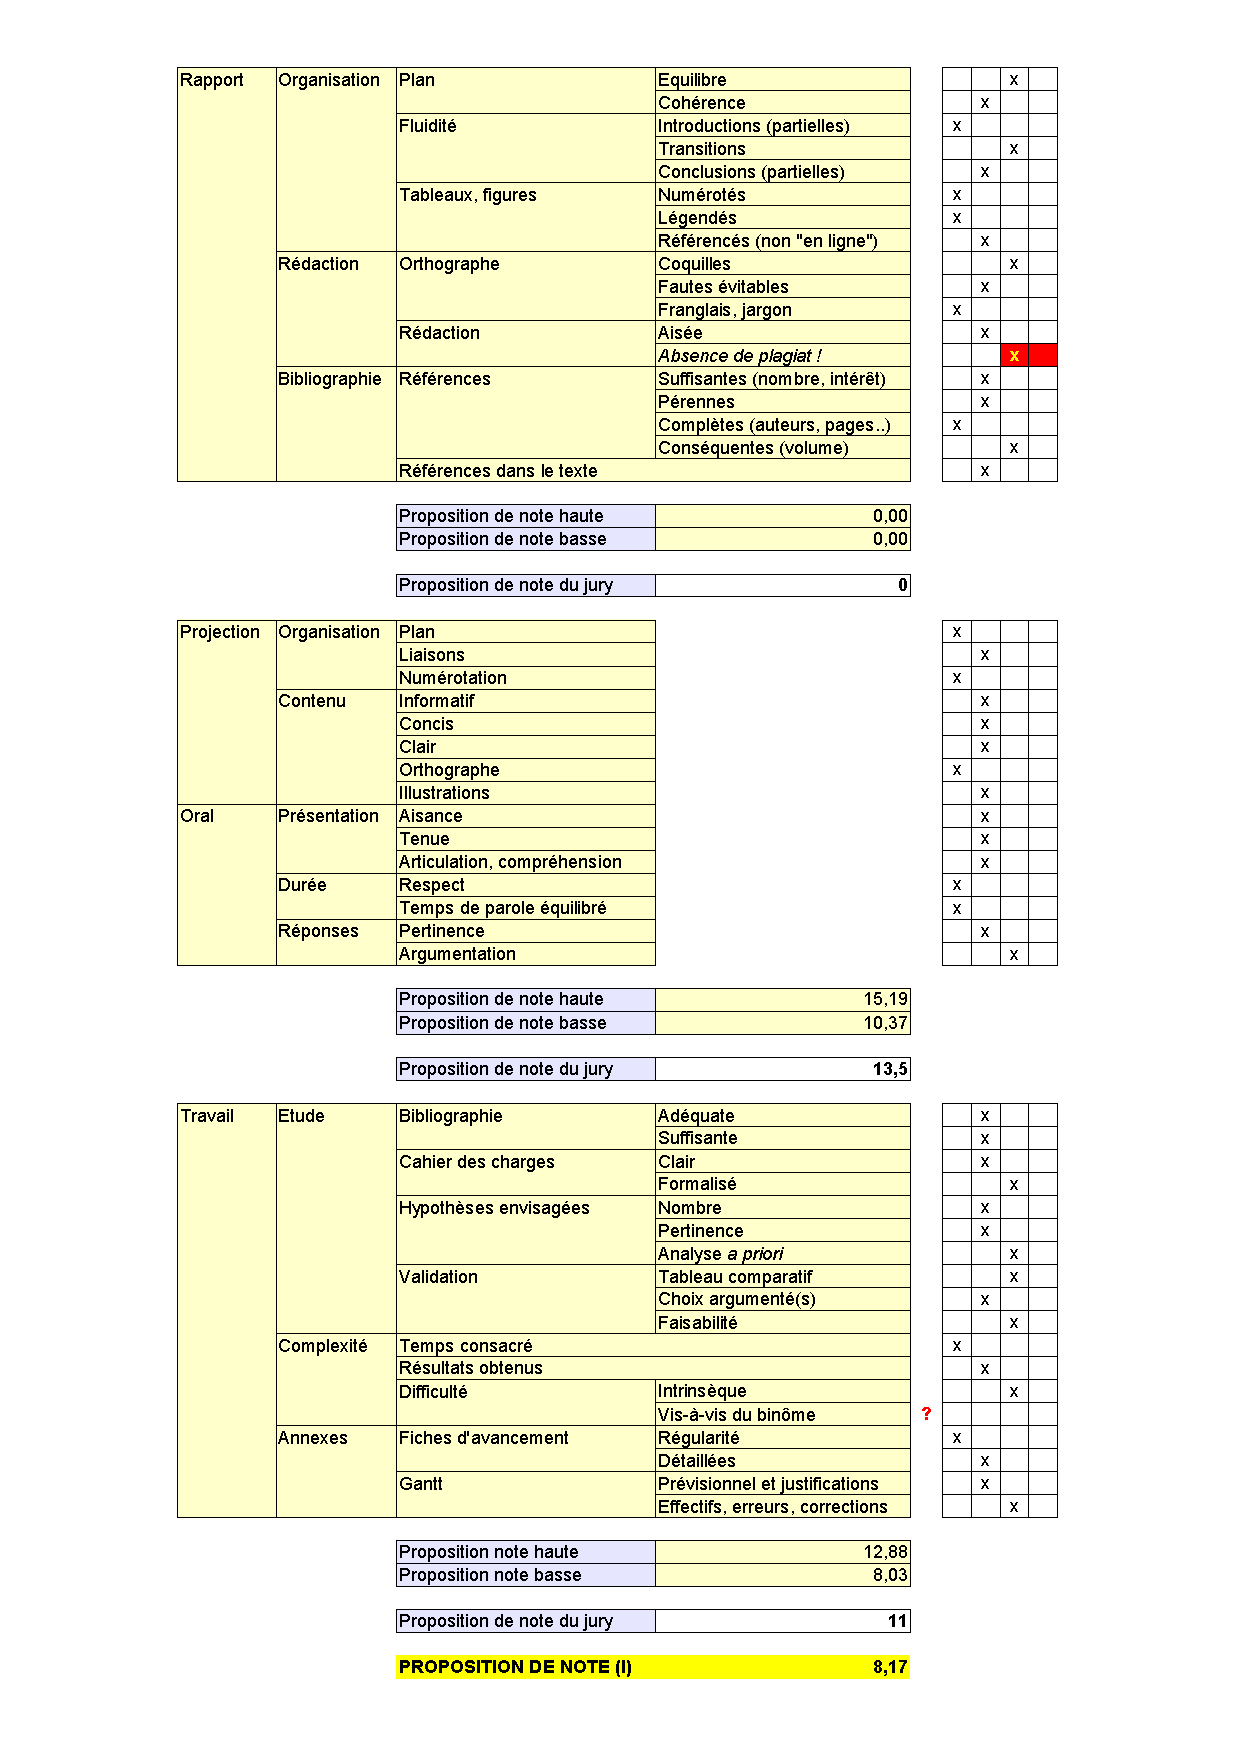
\includegraphics[width=0.9\textheight]{Images/Grille-Evaluation-PRD1}}
      %\else
         %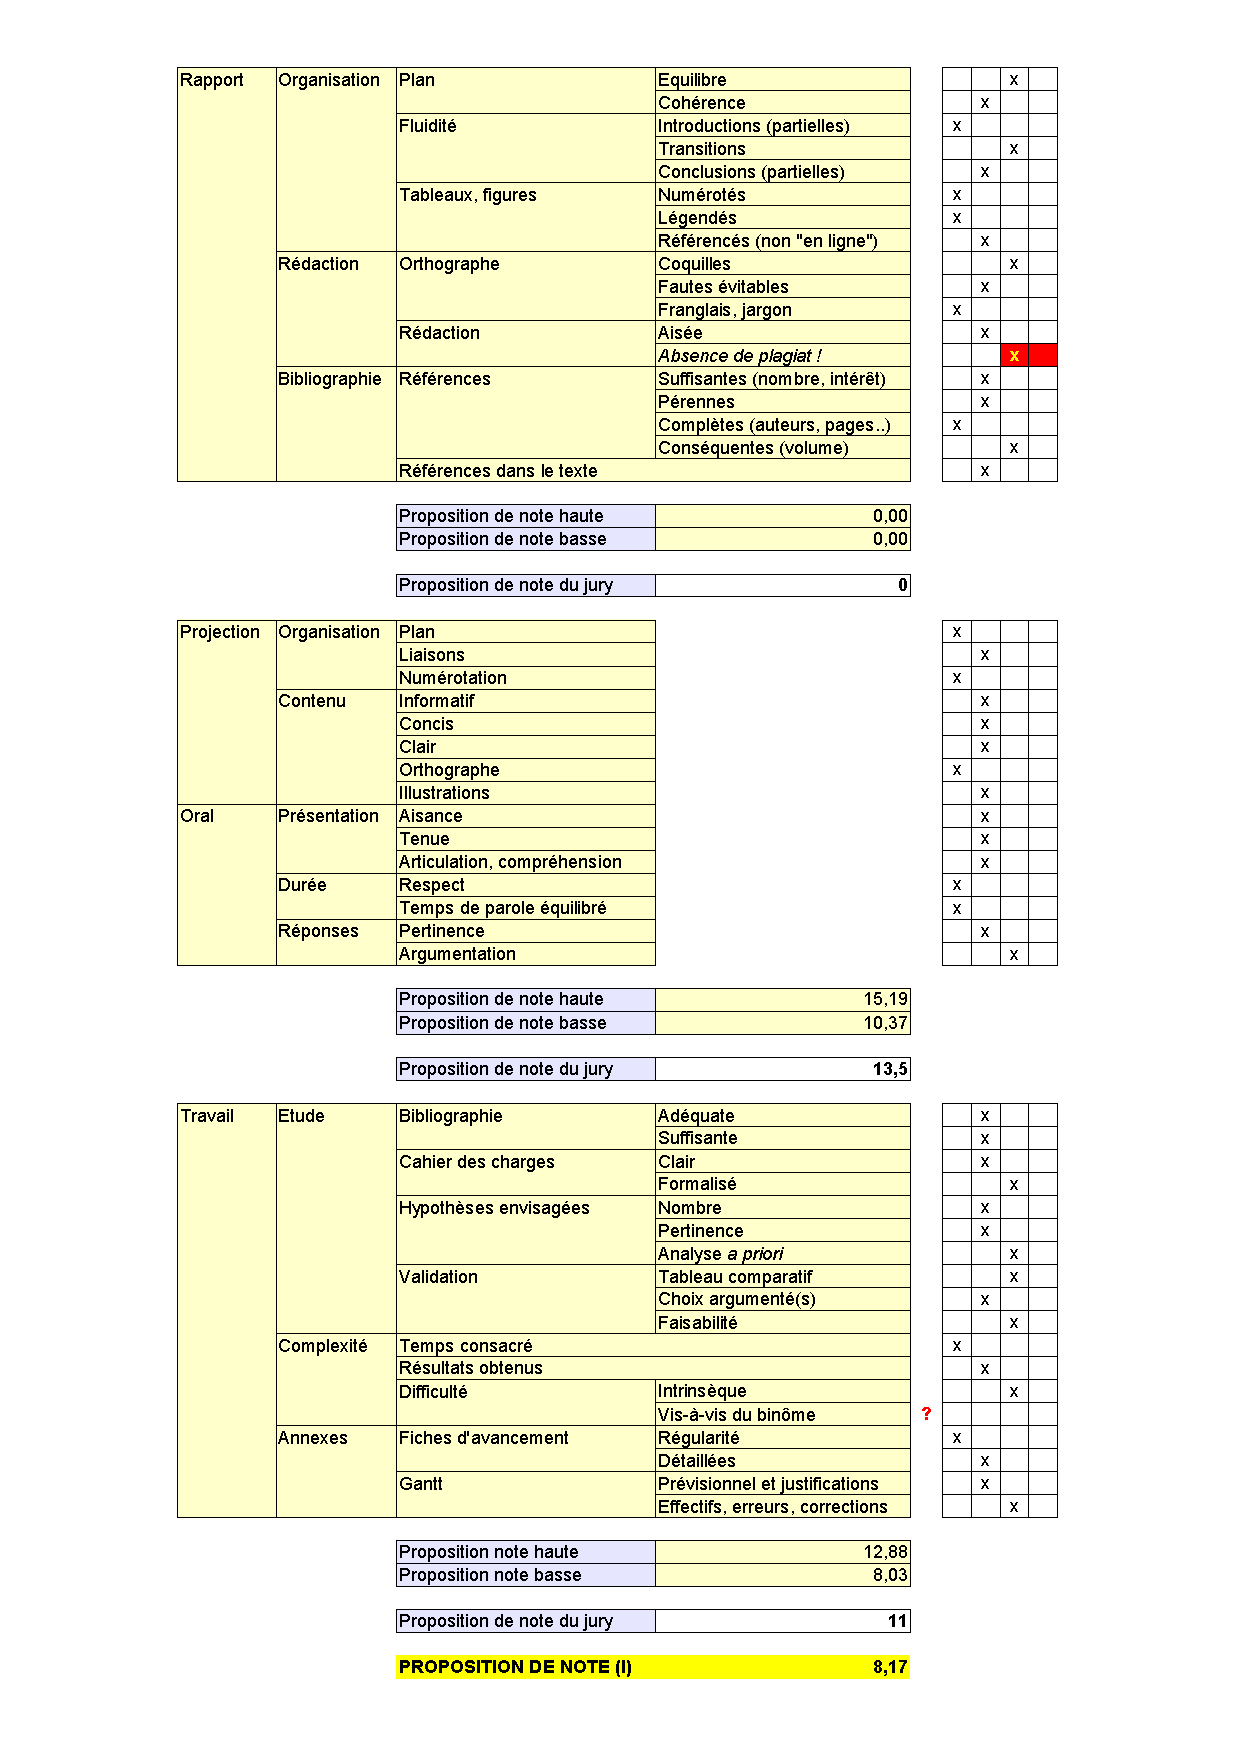
\includegraphics[width=0.9\textwidth]{Images/Grille-Evaluation-PRD1}
      %\fi
 %  \caption{Points � contr�ler � l'issue de la phase I}
 %  \label{fig:IntermediateAutoEvaluation}
%\end{figure*}

%Figure~\ref{fig:FinalAutoEvaluation} provides the same kind of evaluation for the second part of the project, i.e.:
\begin{enumerate}
   \item detailed design;
   \item development;
   \item receipt.
\end{enumerate}

%\begin{figure*}
%   \centering
%      \ifscreen
%         \rotatebox{90}{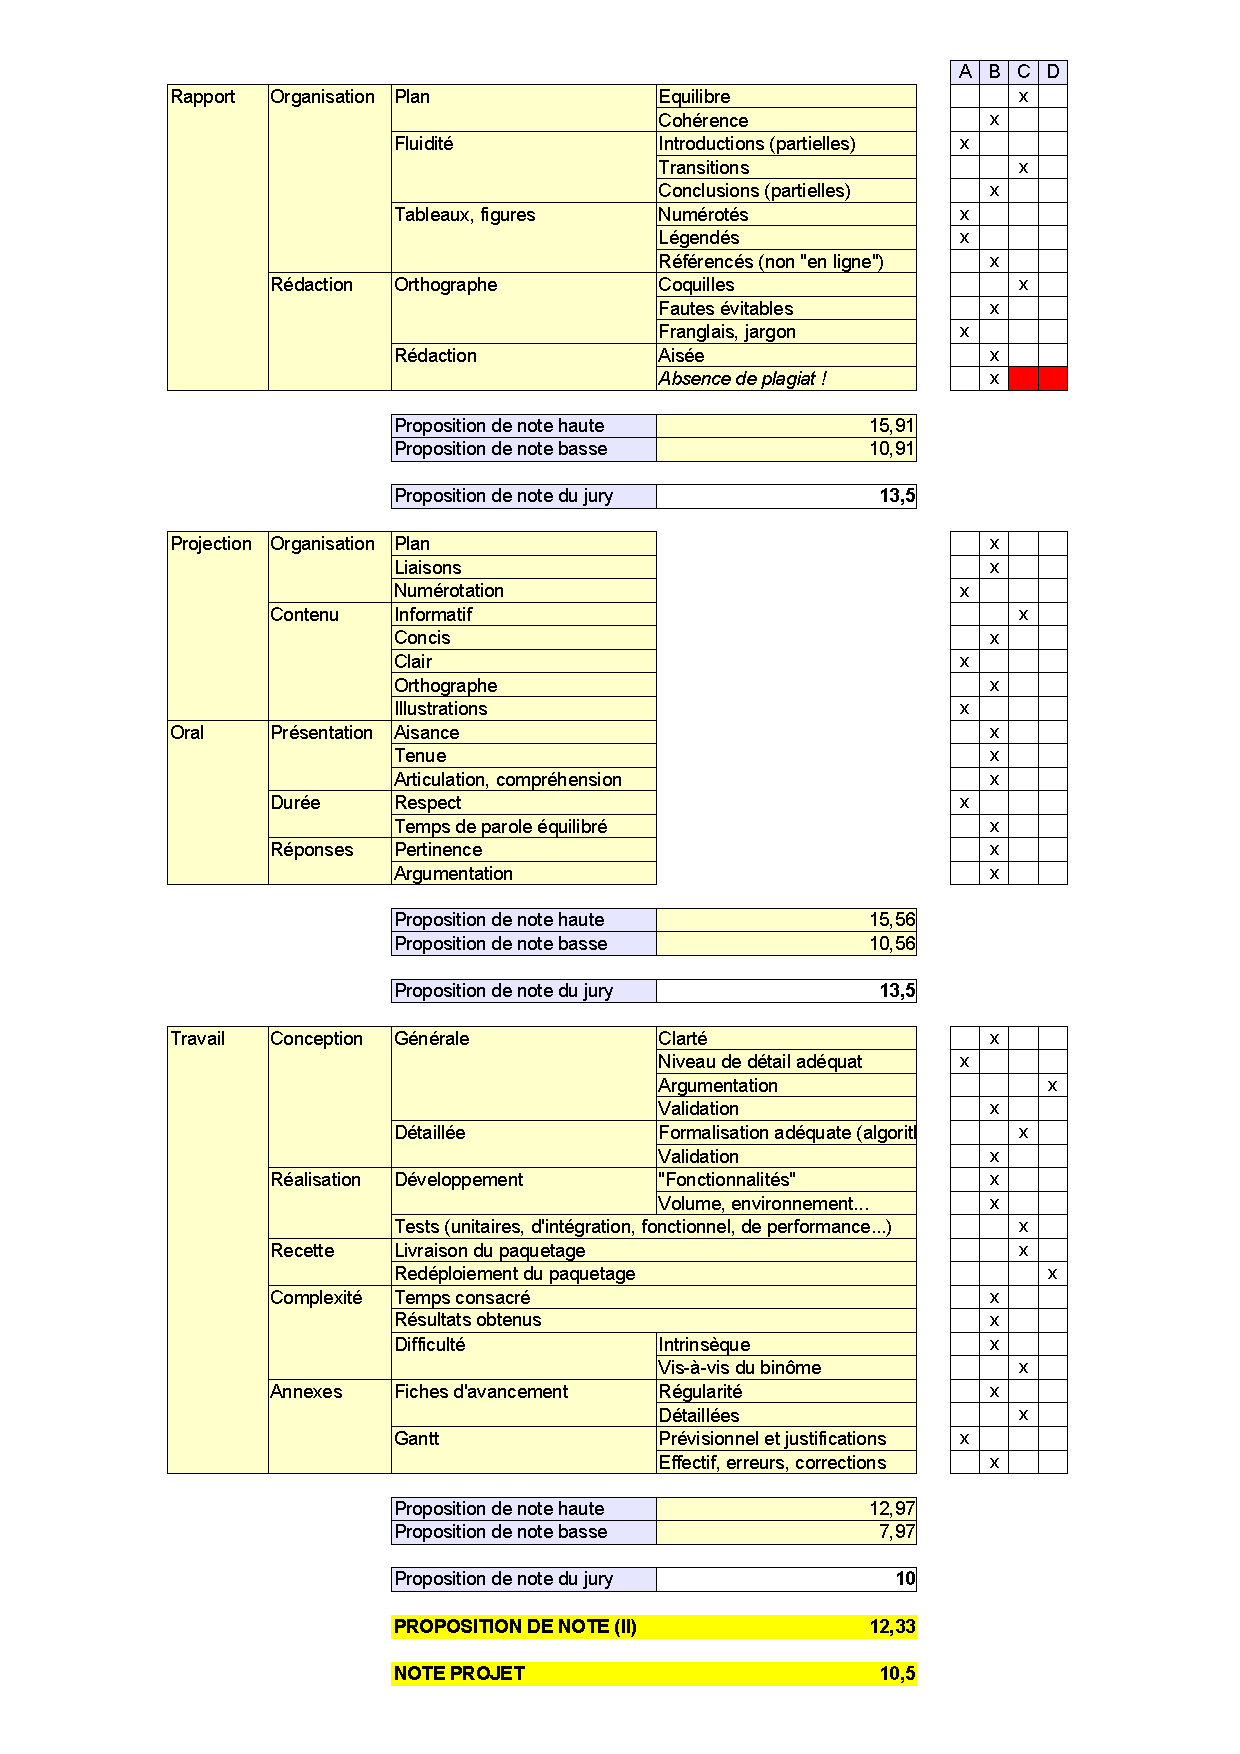
\includegraphics[width=0.9\textheight]{Images/Grille-Evaluation-PRD2}}
%      \else
%         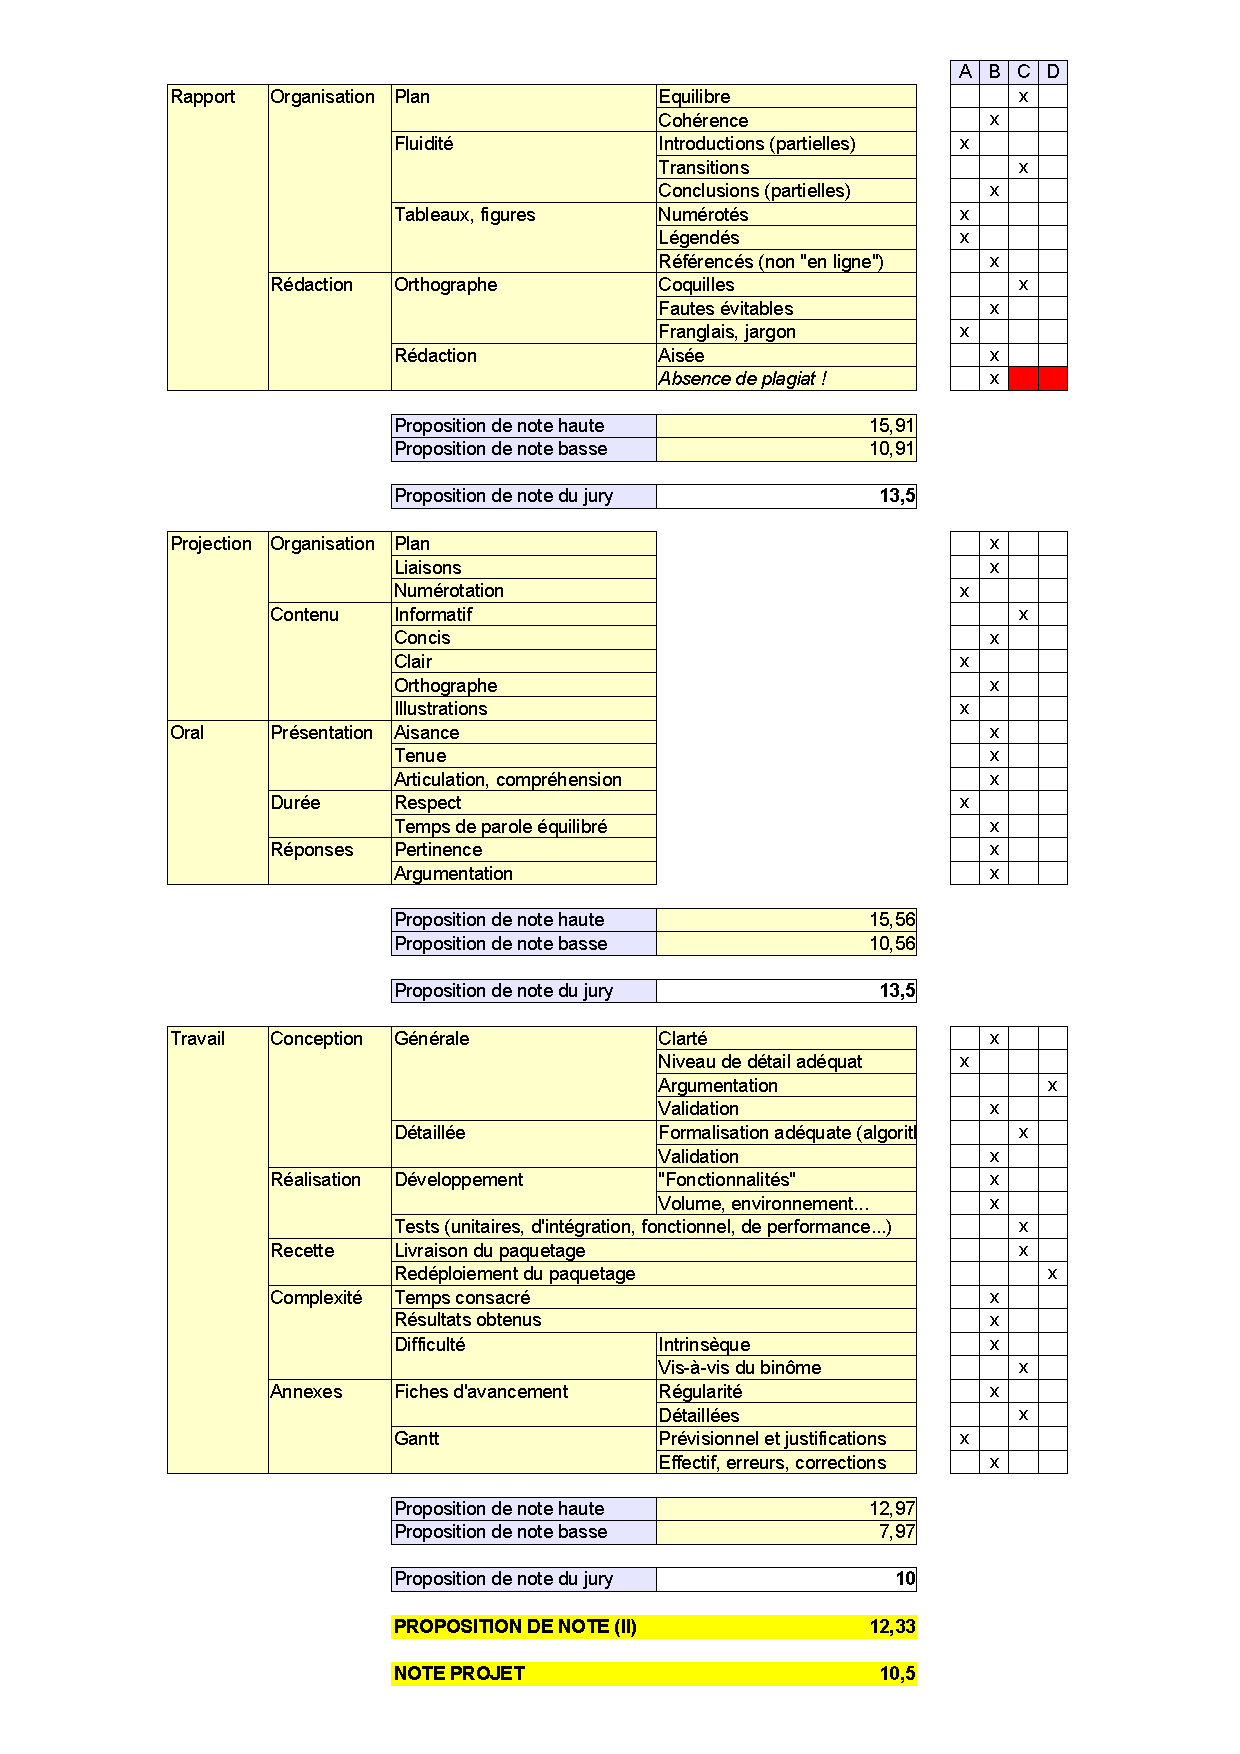
\includegraphics[width=0.9\textwidth]{Images/Grille-Evaluation-PRD2}
%      \fi
%   \caption{Points � contr�ler � l'issue de la phase II}
%   \label{fig:FinalAutoEvaluation}
%\end{figure*}

\end{document}
